\subsection{ Overview Extending Dataset}

The idea is to include more questions about the same objects and the scenes found in EQA-v1. The question generation copies the EQA data-set and modify the so called-episodes in it. The episodes, as mentioned in previous sections, are executable functions when inserted in an environment they yield an answer. The scenes denote the visual scene of the destination goal of the a navigational episode. The system learns to reach its navigational goal by a shortest path included in each EQA-V1 episode. Our new questions use the same shortest path found in EQA-V1. 

This project consist of two major module-components. The first module is a parser that does data extraction, and acts as a processor for raw data by transforming into usable geometric information for generating question-answers. The second module is the question-answer generator. This chapter describes the projects construct and the usage of each part of it.  



\subsection{First module- Data parser}

Our house parser consist of two classes. The first class is a class that parses the houses into a structural data. The second is functional class we use to find near objects close to a target object. The latter class is used 

The experiment include used two different ways for annotation extraction. The first source-method is the raw annotations given in the 'house files' of the MP3D data-set. The second method uses Habitat's simulator and sensors. The annotations extracted from the sensors in the Habitat's simulated environments provide more computed information and slightly different raw data MP3D annotations; In particular, some object names are different, but the rest of information, such as object ids and location-centers, is consistent with the annotation of the MP3D. 

In the existing generated question-answers data-set we use the data extracted from the Habitat semantic sensors. The main reason for choosing Habitat's semantic sensors is because they provide a computed geometric information of the objects such as the location of an object within an Axis Oriented Bounding Box (We elaborate on this term in the coming section). An additional important reason for this choice of extraction is that some of  objects names output-ed by the sensors are aligning with the names found in the original EQA-V1 data-set. For example, object names in MP3D such as l-shaped sofa and rounded-sofa are transformed, in Habitat's sensor, into their Hypernym category 'sofa'. Choosing object names that are aligning with names found EQA-v1, is helpful for having the overall data consistent with each other when we emerge our generated questions with EQA-V1. 

The second major component - get close distances 


\subsubsection{Annotations from MP3D files}


We extract two types of raw information from each object's line of annotation found in the house files in Matter-port. Lines mentioned erlier: [px py pz  a0x a0y a0z  a1x a1y a1z  r0 r1 r2 0 0 0 0 0 0 0 0 ] 

First we take the obj and room indexes (ids). Second is the [px py pz] and where we categorize it as the center of the object's box. Third is the [r0 r1 r2] (radius-half-extent).

we structure the data in a form that the annotation of a house begins with the first level in it, followed by the rooms and objects in each room as: house 1 [{level1:room1[bedroom]:(obj1:bed,obj2:..),room2:(obj..)},, {level2:......} ]  

\subsubsection{Annotation extraction using from Habitat's sensors}

Our final choice for extracting semantic annotations is Habitat's simulator. Our annotation's parser of the houses uses the sensors with configuration provided by the habitat platform \footnote{url{https://aihabitat.org/docs/habitat-lab/habitat-sim-demo.html#scene-semantic-annotations}.}. The configurations include the settings such as the scene, the height and width of the sensors, and the types of sensors to include. color sensor, semantic sensor and depth sensors are used. 

Once we simulate the environment, the sensors output the annotations of a house(scene) as an object. We iterate through the object to obtain information about the levels, rooms, and the objects in the rooms. We freeze the simulator once the annotations' object of one environment is outputted, then repeat the process for the other environments. 

The data about the an environment's annotations include a calculated geometric information. The sensors in the simulator gives an advantage by calculating the sizes of both the AABB and the OOBB. We use the sizes of the OOBB and AABB, to further obtain more specific information about the object's boxes. 


\begin{figure}[H]
\centering
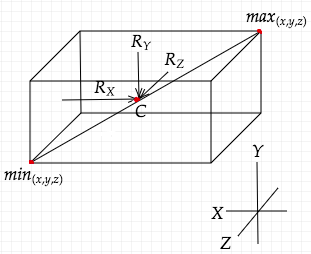
\includegraphics[scale=0.5]{images/Geoinfo.png}
\caption{Min and Max of an Axis Orients bounding box}
\label{fig:aabb}
\end{figure}


We make calculations from the data we extract in order to obtain other necessary info for generating question. Important to mention, the geometric points extracted by habitat's simulator, such as centers of the boxes and the sizes of the boxes' sizes, are represented in 3D data where the  x is the length, y is the width, and z is the height. 

The first calculation is finding the 'min' and 'max' of a bounding box given an object's center and length of its sides on(x,y,z). In figure \ref{fig:aabb} we see visual illustration of the extracted and calculated data. The min represents the corner of a box that has the lowest value of (x,y,z) and max is the corner with largest value for (x,y,z). Other way to put it, the min represents the corner point in the minus direction from the center in all the axis , and max is the corner on the positive direction from the center in all axis. 
%$\displaystyle
The given size of the box is from the min point to the max point with a 3d value (x,y,z). To get each of the points we first get the half extent of the size such as: \begin{math} Half\ extent\ =(x,y,z) /2\ \end{math}. half extent or (radius) is the point from the center to either the min or max. 

The 'min' is the point stretched by the length of the half extent in the negative direction, and 'max' is the stretch to the positive as the following:   \\ 
\begin{math}
Min\ point\ =\ C\ -\ \vec{H} \ \ =\ ( x\_{1} +x\_{2} ,y\_{1} +y\_{2} ,z\_{1} +z\_{2}{}) \  \\
Max\ point\ =\ C\ +\ \vec{H} \ \ =\ ( x\_{1} -x\_{2} ,y\_{1} -y\_{2} ,z\_{1} -z\_{2}{}) \ 
\end{math}

The min and max help us in define spatial relations among objects. How we use them is explained in the coming sections.

We use the OOBB sizes for calculating the sizes of the objects. We consider the size as the volume of the box which is the length multiplied with the height and width. In our case the length is the x value, width is the y value and z is the height, then  the calculated volume of a box is \begin{math} X\ x\ Y\ x\ Z \end{math}. 


We structure the annotations and save them in a file. The structure of the data consist of a dictionary storing the data in a hierarchical way. At the top part is the house id, then rooms in the house, then the objects in the house. Each object stored by id, contains the min and max value of its box, size of its aabb, its name, room name and id where its located, and the level id where the room is located. Storing the annotations this way allows to access all the objects in a room through the scene id and room id. 

 We store the calculated volume of each object in all the houses and store it in a second file. The volumes of objects are stored by their object category. In the volumes file, we find the volumes of all the objects in all of the houses stored in a dictionary, each key represents a category such as 'sofa' with values of the volumes of this object type. The point here is to obtain data on the sizes of each object type. We use this information for finding ground truth answers about for the size questions.  
 

\subsubsection{Second class - Distance and size calculator}

The main functionality of this class is to find a spatial relation between pairs of objects in a room. It takes as an argument scene and room id and uses this information to access the objects in a room from the parsed houses files. 

It outputs three types of spatial relations between a pair of objects. The pairs spatial relation is specified by whether an object is 'on' , 'next' or in unspecified 'close' distance to a second object. The pairs are organized in a dictionary, one key for each spatial relation. This information is used for generating positive spatial questions. 

The spatial relations mentioned above are measured by calculating the distance between the corners of the objects' bounding boxes along certain dimensions. The corners obtained using the 'min' and 'max'. If we iterate over the Min(x,y,z) and Max(x,y,z) we get the other six corners of the box. Figure \ref{fig:box_points} illustrates the eight corners, the view point of the cube is rotated to the right for the sake of viewing all the points in the cube. If we move our point of view directly in front of the cube as if  we are facing the square GHED,  the points A and H would seem to be lying on a straight line. Lying on the same straight line, for example, means the point A and H are located on the same points in the x-axis, and so one for the other parallel points .\begin{figure}[H]
\centering
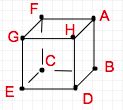
\includegraphics{images/cornerPoints.png} %[scale=0.5]
\caption{}
\label{fig:box_points}
\end{figure} 

We get the rest of points from the Min and Max of an AABB for the reason that AABB's are not rotated and aligning with the global view. To express it better, we image the global point of view of the AABBS as a view facing a group of adjusted and not rotated boxes. 

For our example in figure \ref{fig:box_points}, the values of the six corners of the box found from the Max and Min in addition to the corners of the Min and Max would be as such: 

$\begin{array}{l}
A\ =( x_{max} ,Y_{max,} Z_{max}) ,F=\ ( x_{min} ,Y_{max,} Z_{max}) ,H\ =\ ( x_{max} ,Y_{min,} Z_{max}) ,\\
B=( x_{max} ,Y_{max,} Z_{min}) ,D=\ ( x_{max} ,Y_{min,} Z_{min}) ,\ C=( x_{min} ,Y_{max,} Z_{min}) ,\\
G=\ ( x_{min} ,Y_{min,} Z_{max}) ,\ E\ =( x_{min} ,Y_{min,} Z_{min})
\end{array}$

  


A visual representations of the corners and their values seen in figure.X 


The definition of each of the mentioned spatial relation , is an approximation of how we define them as humans. Each of the spatial relations are determined given a geometric criteria of distances and positions between objects' corners along the three axis  (x,y,z). 

Two general operations are used in each of the relations. The first one is calculating  the Euclidean distance between two corner points; denoted as the distance between p and q in this formula:  \begin{math}
 d\left( p,q\right)   = \sqrt {\sum _{i=1}^{n}  \left( q_{i}-p_{i}\right)^2 } 
 \end{math}

The corners, depending on the type of relation we want to extract, can be represented as points in  1d, 2d, or 3d. 1D is  when we pick points from one of the axis only. 2D is a point on two axis, and 3D is a point on three axis as the corner examples illustrated earlier. We describe this in more detail in the sections below. The second operation is calculating if one of side of a box on a certain axis is contained within the other. 

\begin{figure}[H]
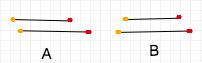
\includegraphics[scale=0.5]{images/contained.png}
\caption{}
\label{fig:contained}
\end{figure}

The calculation if one side is contained within the other relies on defined criteria. The calculation is done in a specific function and  can take as input  corner points on one axis or more. In the drawing \ref{fig:contained} 'A' represents two lines on the 'X' axis where the top part is not contained within the other, an in 'B' the top is contained within the lower line. In this example we determine the 'contain' relation by taking the 'min' represented by the the orange dot and the 'max' doted in red. 

If the min of the upper line is greater than the min of the lower line and the max of the upper line is less than the max of the lower line then the upper line is contained within the lower. Hence the 'min' of the upper line is greater than the 'min' of the lower line because it's more to the right in the positive direction of the 'x' axis. If the previous condition is not satisfied, then the lines are otherwise not contained. 


The operations above are done over different axis for every relation. Below we specify how each of the 'on', 'next to', and 'close' relation is determined between the objects. 

\paragraph{On}



First step is choosing pairs of objects that are closest to each other vertically(on the Z axis). The distance should be less than a 0.5 millimeter thresh hold. The Euclidean distance here is calculated between the 1D points on the Z axis only. Two corner values from each box and any corner match the distance required are picked out. 

\begin{figure}[H]
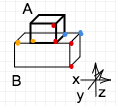
\includegraphics[scale=0.7]{images/on.png}
\caption{}
\label{fig:on}
\end{figure}


The second step consist of a group of conditions that the pair of objects need to meet in order to be considered on each other. The first condition is that the vertical sides, the line from Zmin to Zmax, of the boxes are not contained within each other. The Zmin-Zmax lines of every object box are the lines between the two red dots in box A ans B in the illustration \ref{fig:on}. Otherwise if the lines on the Z axis are contained it would mean one object is inside the other. 

The second condition is that the horizontal line of one of the boxes is contained within each other.The horizontal lines in the illustration are from the Orange to the red points in each box. The lines on the y axis from the red to the blue points should also be contained. 

The final step is deciding which object is on the top of the other. The pair of objects are passed to a function that see which Zmin-Zmax has greater value. The object on the top should be in the upward positive direction. 


\paragraph{next to}


\begin{figure}[H]
\centering
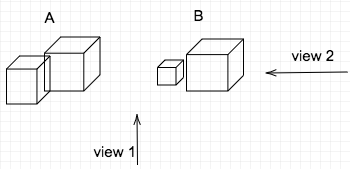
\includegraphics[scale=0.5]{images/Nextview.png}
\caption{}
\label{fig:next}
\end{figure}


A pair of objects next to each other have to have a distance not greater than 0.1 meters on the X and Y axis. The distance here is calculated for 2D corner points, this means the distance is calculated for four corners (min and max front and back).

The pairs should not have contained sides in neither the x nor the y axis. In this condition a pair of objects next to each other would like illustration A in \ref{fig:next}. This is might a bit different from what we consider next to each other as humans. We might imagine a typical next to pair as illustration B seen from view 1.

However, the choice of having 'next to' pairs not contained with each other is due to considerations of the view point. From view 1 the pair(B) seem next to each other but from view 2 they would not. In pair(B) from view 2, one object would be behind the other and likely hidden. So if view 1 is the global view and we pair the objects as in (B), seen as next to in view 1, the robot might enter the scene from view 2 and it would be wrong to refer to the pair as next to each other. However, if the 'next to' pairs are assigned as in illustration (A), the pair would be still visible in whichever view, and positioned proper enough to be referred to as next to each other. 

Finally the pair must have their lines contained on the Z axis. Otherwise, the two objects might satisfy the first condition on the (x,y) but be distant on the z axis, such as one object in the ceiling and the other on the floor. 


\paragraph{close to}

A pair close to each other are a pair who has any of their 3D corners close to each other within a max distance of 0.2 meter. No other conditions required for the pairing of objects close to each other. It can be a close object on, above, below or next to. 

\subsection{Second Module - question generation}


\begin{figure}[H]
\centering
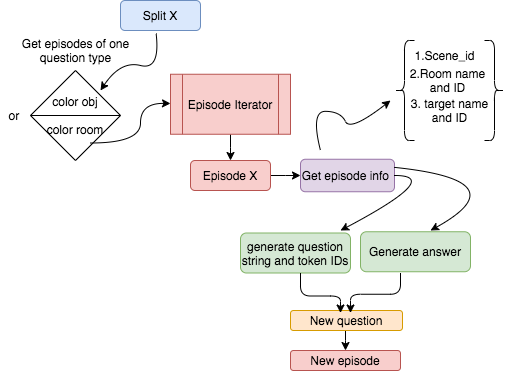
\includegraphics[scale=0.5]{images/generator.png}
\caption{Split generator}
\label{fig:generator}
\end{figure}



 Our question generator generates questions of two types, size and spatial. In order to run the generator, the arguments required are the type of question, path to the val and train splits. 


 The question generator generates questions of one type at the time. Questions with the string "room" in is considered a different type from a question that refers to objects without a room. For example, the question "How big is the table?" has the type "Size", and the question "How big the table in the living-room?" is of type "Size room". In order to generate size questions with and without reference to a room, therefore, requires ruining the code, one separate time for each type. 

The split generator is the core component in the code. It takes a split either train/val and a question-type as arguments. The functionality of the split generator is to turn an EQA v1 split of episodes into a new split of new episodes. In figure \ref{fig:generator} we see an illustration of the workflow of the split generator. The five general steps is filtering(uncolored rotated square), iterator(red rectangle), episode parser (pink rectangle),  QA generator (the green rectangles), and  episode wrapper (the bottom yellow rectangle- inputs QA and outputs episode )  

The filter returns a set of question-episodes of one type only. The returned set of questions of a type is dependent on the question type given to generate. For example, if the input is to generate questions of 'size-room', 'how big is the sofa in the room', we take only the questions of "color-room" type. 

The filtered set is passed to an iterator. Each iteration passes one episode from EQA-v1 to a parser. The parser function in the iterator extract information, such as the object name and id, scene ID and room ID, from the EQA-V1 episode. 

The parsed information is passed to a QA generator. The QA generator is better described  as a group functions of the split-generator that are conditioned differently dependent on the question type. The answer generation function is, however, a different function for each question type.  

 The general idea for generating QA of any type relies on two straightforward steps. First, generating a ground-truth answer for the given question, which is the most important stage in the generation process as it requires calculating values from the data in the houses. Second step generating a question string and token ID's.

The  final step consists of inserting the new question with the corresponding geometric information, and structuring them into an executable function.  We call a QA sample an episode when the section of the episode seen in figure \ref{fig:episode} are filled with the new QA and the other the corresponding information. 

Our question generation can be described as generating one question for every “shortest path” there is. The idea of transforming  an episode from EQA into a new one is based on using the starting position and the 'shortest path' found in them. Having more questions for each shortest path is equivalent to having multiple questions about the same scene. 

\begin{figure}[H]
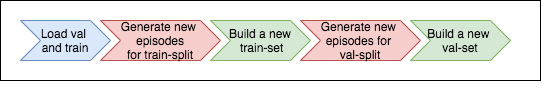
\includegraphics[scale=0.5]{images/stages.png}
\caption{Split generator (The top part of the code)}
\label{fig:stages}
\end{figure}


The top most part of the code (the data-set generator), illustrated in figure\ref{fig:stages} , passes the train and val to the split generator at different time-stamps. The reason for generating the two splits in two different stages is to keep track of the number of question-answers generated for each split. Emerging the two splits and splitting them randomly at the end might create and imbalance between the  answers in each split. The current code controls the distribution of answers in the train and val sets. Otherwise, leaving the type of answers uncontrolled would leave a bias towards one answer over the other. 

Once a split of episodes is generated it's passed to loader function. The loader function inserts the answer and question vocab to finalize the data-set in the form seen in figure 2.2

 In the coming two sub-section we describe in detail how the QA generators for the size and spatial questions work. 

\subsubsection{size-questions}

Size questions are generated through three steps. The first step is generating a ground truth answer about the size of the the target-object found in EQA-V1 episode. There three possible answers are  Big, Small, and Medium. The second step is generating a question string and token ids. The final step consist of filling the question-answer in an episode form, with shortest path and the rest of object's info from the original EQA-v1 episode, as described in the previous section. 

\subsubsection{Size answer} 

The size answer is generated in a function referred to as "GetsizeAnswer". This function takes as an argument the target-object's name and the size of its box and returns an answer about its size. The function calculates the volume of the target object in a similar way as the rest of the sizes of the objects. Volume of the OOBB = W x L x H. The next step in the function is to compare the size of the target to the sizes of the objects of its type.

The relative size is determined by its deviation from the standard of its type. As mentioned earlier the sizes of all objects are stored by type in a file. We pick the volumes of the object's type and calculate the mean size and the standard deviation of all the the sizes from the mean. The standard deviation denoted below: 

\[ s = \sqrt{\frac{1}{N-1} \sum_{i=1}^N (x_i - \overline{x})^2} 
\]

The answer is 'small' if the objects' size is smaller the mean size of its type minus the standard deviation,  'big' if the size is larger the median + the standard deviation, and middle if the size of the object is within the standard deviation added and subtracted from median. 

We control the answers' distribution. We observe that a majority of objects have a medium size given the standard of their type. In order to avoid bias towards the 'medium' answer, we restrict the number of QA with medium answer. We keep track of how many QA with medium answers has been generated and when the number reaches a limit we generate None QA that are later filtered out. The limit varies depending on the question type and the split (train or val), and is based on our observation of the answer distribution in the splits. Note that we refer to 'question type' in this example if either the question to be generated is size question with string 'room' such as "color-room" or without. 


\paragraph{question-string}

The question string generator takes a question type, and an object as an argument and returns a complete question string. 

The templates for size questions are as the following: 

size\_obj : 'how big <AUX> the <OBJ> ? \\
size\_room:'how big <AUX>  the <OBJ> in the <ROOM>?'

\subsubsection{spatial-questions}

Generating spatial question takes more complex steps and longer time than generating size questions. Generating a spatial QA requires a coordination with the spatial relation extractor. In addition, spatial questions include the addition of an extra object to the question string, and the insertion of the new object's information into the QA episode. 

Searching for spatial relations of the target object in an EQA episode is the first step taken. We pass the scene an room id to the 'relation' extractor to obtain pairs of objects, within a room,  with a spatial relation between them. The relation extractor returns three types of relational : next, on, or close, if existent within a room. Else it returns a category with empty values. 

The decision of generating a question of one of the mentioned relational categories is dependent on the existent of an object with a spatial relation to the target object. The process of executing a generation command of a question of a spatial type is illustrated in figure \ref{fig:spatial}. If there is an object 'on' the target or a target is on another object, we generate one questions, and similar case if there is an object next to the target object. If there is no 'on' or 'next' relation or either of them is non existent, the criteria for checking if there is a 'close' object is satisfied. If none of the conditions are satisfied a QA with no 'answer' of a random spatial type is generated.   

\begin{figure}[h]
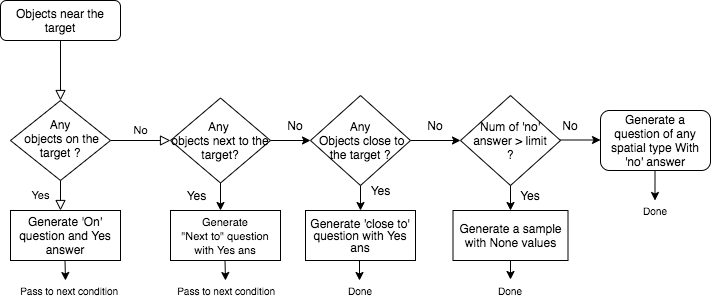
\includegraphics[scale=0.4]{images/spatialconditions.png} %[scale=0.2]
\caption{Decision tree for generating different types of spatial questions}
\label{fig:spatial}
\end{figure}

A QA with positive spatial answer has a 'yes' answer, and 'no' if a relation is non existent. The decision tree as seen \label{fig:spatial} leverages positive QA for the reason that we observe that the no-relation instances outnumber the positive ones. The final condition, we even control the number of QA with 'no' answer by generating a None QA if the number of generated QA with no answer reaches a limit. The QAs' with None values are later filtered out.

Within this decision structure, for each 'shortest path' in an EQA episode, there is a possibility for generating from one to two spatial questions of different spatial type. 

The process of generating a spatial question includes the addition of information about two objects. An episode/question generator, a group of functions, adjust itself to a spatial question generation if certain arguments are given to it. These arguments are seen in the input section  in the illustration in fig \ref{fig:spatialGen}. Such as potential  object type, spatial question type, and all object in a room 

\begin{figure}[h]
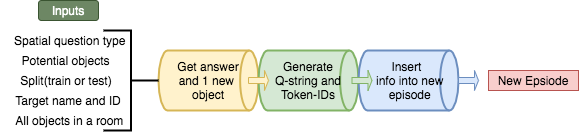
\includegraphics[scale=0.4]{images/spatialGenerator.png} %[scale=0.2]
\caption{Structure of spatial questions generator}
\label{fig:spatialGen}
\end{figure}

All the inputs seen in \ref{fig:spatialGen} are required to generate an answer from a function called "GetSpatialAnswer". All objects in a room are needed for generating "no" answer. In case of generating a "no" answer the "GetSpatialAnswer" function picks a random object fro the houses that is not in the room. The reason of excluding objects in the room from the selection of a random object for a negative QA is to help us in the validation process, such as we would know if the robot answer 'yes' to a QA with 'no' as ground truth that it's due to bias rather than he robot recognizing the object in the scene. 

A selected object of potential objects and the type of spatial question are required arguments for generating spatial question string and token ids. 

The last part in blue is conditioned by the type of answer, if it's 'yes' or 'no'. If the answer is yes, geometric information of the target object's pair is passed to it to insert it in the episode. If the answer is 'no', no additional information is added to the episode beside the information of the target object found at the end of the shortest path. 
\paragraph{Question strings}

To generate a spatial question string, the string generator takes as an argument the question type such as "spatial\_room" and and spatial relation type such as "on", "next" or "close". The string templates are the following: 

'<AUX> there <ARTICLE> <OBJ1> close to the <OBJ> in the <ROOM>?'/\\
'<AUX> there <ARTICLE>  <OBJ1> next to the <OBJ> in the <ROOM>?' \\
'<AUX>  there <ARTICLE> <OBJ1> on the <OBJ> in the <ROOM>?\\
'<AUX> there <ARTICLE> <OBJ1> close to the <OBJ>?',\\
'<AUX>  there <ARTICLE> <OBJ1> next to the <OBJ> ?',\\
'<AUX>  there <ARTICLE> <OBJ1> on the <OBJ>?'


\subsection{Results}

\subsubsection{Total number of generated questions}

\begin{figure}[H]
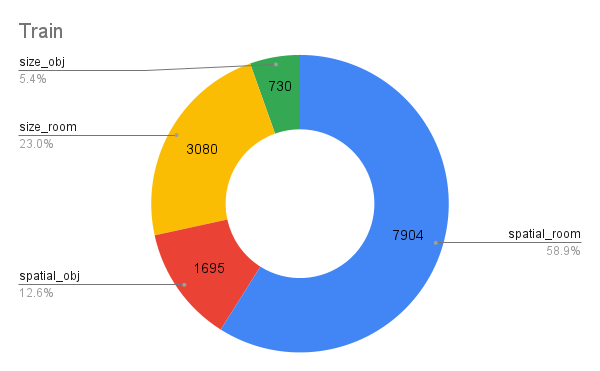
\includegraphics[scale=0.25]{images/GenTrain.png}
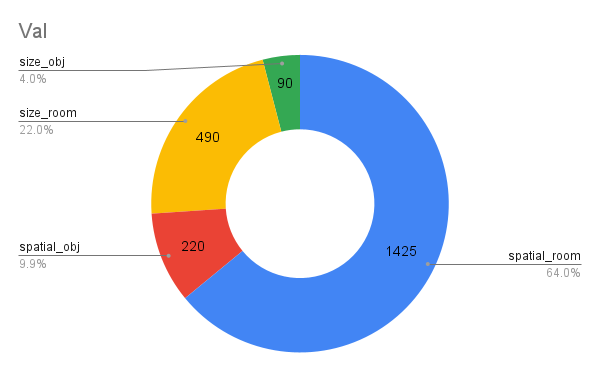
\includegraphics[scale=0.25]{images/GenVal.png}
\caption{}
\label{fig:questionGen}
\end{figure}

We generate a total of 13 409 question for train and 2 335 questions for validation.  In figure \ref{questionGen} questions of size\_room and spatial\_room refer to questions that contains a reference to a room, such as 'How big is the bed in the bedroom?'. Questions of spatial\_obj or size\_obj type are questions with a reference to object only, such as "Is there a chair next to the table?". 

\subsubsection{Answers distribution}

\paragraph{Answers distribution of spatial questions}

\begin{figure}[H]
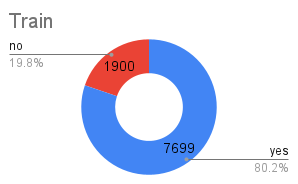
\includegraphics[scale=0.45]{latex/images/TrAnSp.png}
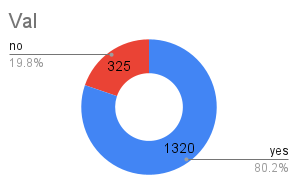
\includegraphics[scale=0.45]{latex/images/VlAnSp.png}
\label{fig:AnsDist}
\caption{}
\end{figure}

The majority of answers for the spatial questions are positive "yes" as seen in figure \ref{fig:AnsDist}. This imbalanced distribution is an intended outcome. The motivation behind this intention is based on an idea, formulated by \cite{regier1996human}, of learning of positive samples only. The argument behind this approach to learning  is inspired from a cognitive theory of human's first acquisition of language. The theory is  based on the premise that humans tend to learn spatial relations from positive evidence instead of non existent instances.

\paragraph{Answers distribution of size questions}

\begin{figure}[H]
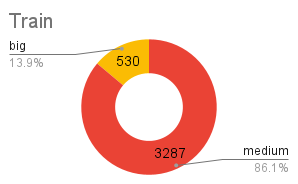
\includegraphics[scale=0.45]{latex/images/TrAnSi.png}
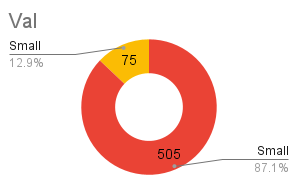
\includegraphics[scale=0.45]{latex/images/VlAnSi.png}
\caption{}
\label{fig:AnsDist}
\end{figure}

The outcomes of generating size questions resulted with zero samples of "small" answer and a majority of 'medium' answer as seen in figure \ref{fig:AnsDist}. In the QA generator, we intended to limit the question-answers with "Medium" answer based on an observation of their dominance. However, limiting the 'medium' answers more than the presented numbers would have resulted in a very few question-answers of size type. An insignificant proportion of size questions was insufficient for training the model . We decided to keep the size questions with their imbalanced distribution, despite knowing that this linguistic bias might hinder the learning outcomes.  

\subsubsection{Discussion}

Our question-answer generation is very dependent on the objects and the shortest paths found in EQA-V1 data-set. The geometric information such as  starting positions and shortest paths are required material for extracting scenes training and testing the VQA model. To be only dependent on the objects found in the EQA restricts our choice over the QA that we could generate. The most prominent limitation we see in the generated questions is the inability to control the answer distribution for size questions. None of the target object's found in EQA V1 turned to be of a small size, based on the criteria we establish for determining an object's size. 

The description of sizes is paradoxical. A well established paradox, in philosophy


Topic sentence: we add spatial questions for the goal of .... deespite haing lingustic bias? 

Evaluation depending on no answers


Our choice to include size and spatial questions is motivated by the belief of the importance of spatial language to cognition. (\cite{landau1993whence}) in “spatial language and spatial cognition” states that the human first acquisition of linguistic names of objects in the physical world is associated with establishing a geometric representation of what defines them. In particular, the conceptual identification of an object might be defined within a spatial relation to other entities, and the image we mentally construct of a concrete noun of a physical property, may appear in the form of its shape.

The annswer 

Our question-answer generation is very dependent on the "shortest paths" in EQA-V1 data-set and the objects they lead to.  



